\section{Materials and Methods}

\subsection{Finite element modelling approach}

The finite element modelling workflow used in this project is a Python-controlled COMSOL Multiphysics pipeline. Model variants are defined in TOML configuration files, from which the pipeline generates source-case settings, COMSOL Java builder scripts, build manifests, solver/post-processing scripts, and summary metrics. The active package is \texttt{ews\_fem\_pipeline\_comsol}. The source-case settings used by COMSOL are now contained inside this package, so normal COMSOL generation, build-only checks, and post-processing do not require the older FEBio-oriented package at runtime.

The older FEBio route remains relevant historically because it provided the original soft-tissue modelling structure and Mooney--Rivlin-style material parameters \cite{BabarendaGamage2017}. In the current work, however, COMSOL is the active implementation route because it supports constructive geometry operations, boolean region definitions, automated selections, and structured post-processing for multiple model variants. The results should therefore be interpreted as controlled model-development comparisons, not as clinical validation against patient-specific measurements.

\subsection{Overall staged pipeline}

The model was developed as a staged COMSOL pipeline so that motion input, anatomical geometry, glandular tissue distribution, support assumptions, and tumor sensitivity could be introduced separately. This was important because the project goal was not to build one final patient-specific model in a single step, but to construct a reproducible model-development route in which each component can be checked before it is used in a dynamic comparison. Figure~\ref{fig:mm_pipeline_overview} summarizes the software workflow from TOML case definition to COMSOL build, solve, post-processing, and report outputs. Figure~\ref{fig:mm_stage_option_overview} summarizes the modelling stages used in the current report.

\begin{figure}[H]
\centering
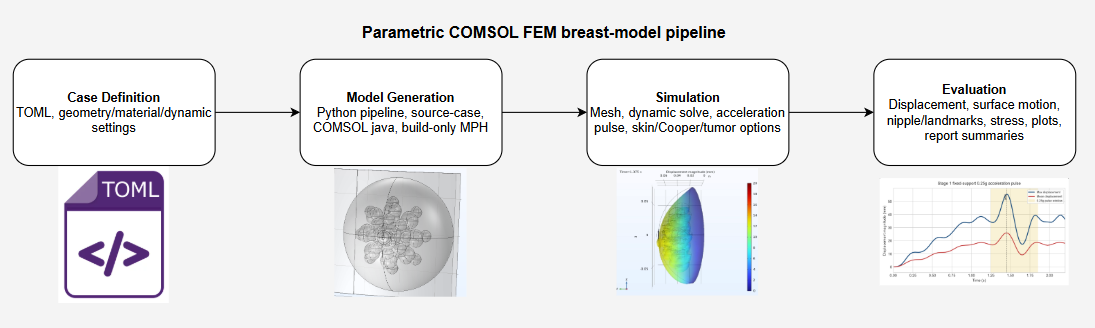
\includegraphics[width=0.95\linewidth]{Figures/model_overviews/model_pipeline_overview.png}
\caption{Overview of the COMSOL EWS FEM pipeline. TOML configuration files define the model variant, after which the Python package generates COMSOL Java builders, build and solve artefacts, post-processing scripts, summary metrics, and report figures.}
\label{fig:mm_pipeline_overview}
\end{figure}

\begin{figure}[H]
\centering
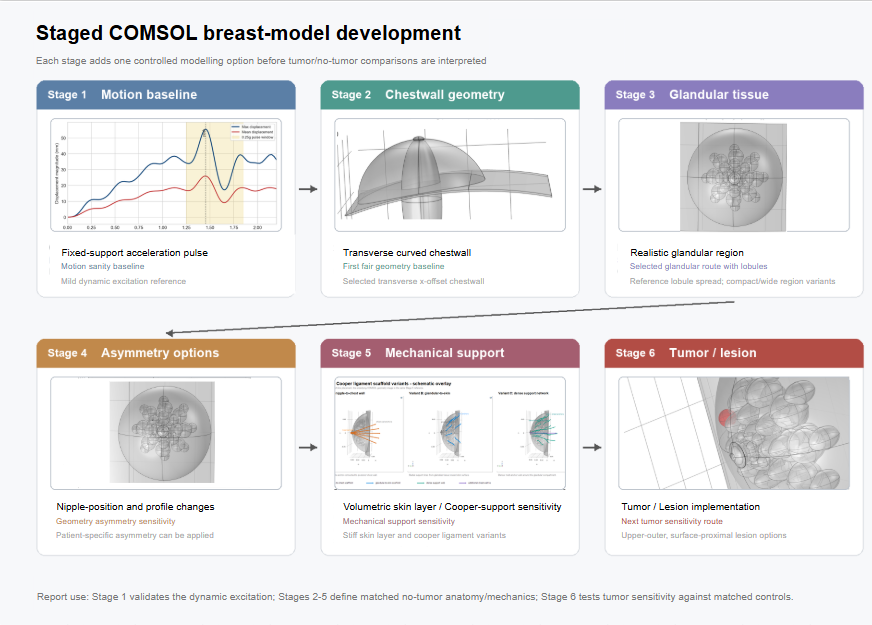
\includegraphics[width=0.95\linewidth]{Figures/model_overviews/Model_stages_overview.png}
\caption{Staged COMSOL breast-model development route. Stage 1 validates the dynamic excitation, Stages 2--5 define matched no-tumor anatomy and mechanics, and Stage 6 adds tumor/lesion sensitivity on top of matched controls.}
\label{fig:mm_stage_option_overview}
\end{figure}

\paragraph{Stage 1: motion sanity baseline.}
Stage 1 was used to test the fixed-support acceleration-pulse input. The selected mild input applies a 0.25g acceleration pulse over 0.60 s after gravity preload with mass damping alpha = 60 s$^{-1}$. This stage is useful for validating the dynamic excitation and checking whether the pipeline produces a clear time-dependent displacement response. It is not used as the final anatomical reference because the geometry, volume, glandular setup, and material context differ from the later matched anatomical route.

\paragraph{Stage 2: chestwall geometry.}
Stage 2 introduced the first fair anatomical geometry baseline. The selected route uses a transverse xoffset055 chestwall curvature with volume-preserving compensation and automatic nipple/gland alignment. Other chestwall variants, including sagittal or combined superior-inferior curvature, are treated as diagnostic geometry checks rather than the current report route.

\paragraph{Stage 3: glandular tissue distribution.}
Stage 3 added a realistic chestwall-aware glandular lobule distribution. The selected reference route increased the glandular fraction to approximately 24.3\% and is anatomically more informative than the earlier simple glandular fraction setup. Compact and wide lobule-spread variants are retained as later spatial-distribution sensitivities.

\paragraph{Stage 4: asymmetry and nipple-position options.}
Stage 4 separates the matched no-asymmetry reference from visible asymmetry and nipple-position sensitivity cases. The current Tier 1 reference intentionally keeps asymmetry disabled so that profile-asymmetry and nipple-shift variants can later be compared against a clean control.

\paragraph{Stage 5: mechanical support and skin-layer development.}
Stage 5 provides the no-Cooper mechanical control and the route for support sensitivity. The current robust control is the no-Cooper case. Cooper ligament scaffolds are still treated as mechanical support sensitivity because stable dynamic Cooper effects have not yet been demonstrated. A volumetric skin layer was subsequently added as a more defensible skin representation than the earlier shell-scaffold route, but its final dynamic effect is still being evaluated.

\paragraph{Stage 6: tumor/lesion sensitivity.}
Stage 6 adds tumor/lesion sensitivity on top of the matched anatomical route. The current implementation uses an analytic spherical tumor-mask material overlay rather than a separate segmented tumor domain. This makes the first Stage 6 route suitable for controlled size, stiffness, and location sensitivity, but not yet for patient-specific tumor reconstruction or clinical diagnostic claims.

\subsection{Geometry modelling}

The breast geometry is parameterized rather than patient-specific. This makes it possible to isolate the effect of controlled model changes, but it should not be presented as a replacement for MRI- or scan-derived patient geometry \cite{Samani2001,Hsu2011,Mazier2024}. The current anatomical route starts from the Stage 2 xoffset055 transverse chestwall case, which has a breast volume of approximately 585 mL. This volume lies in the lower-middle range of the available 100-sample breast-volume dataset and is consistent with using the model as a controlled anatomical baseline rather than as a universal breast shape.

Stage 2 changed the posterior interface from a simple support surface to a transverse width-curved chestwall. Earlier curvature variants were useful for development but were not used as the final anatomical route because they changed breast volume too strongly. The selected xoffset055 case uses volume-preserving compensation and auto-alignment of the nipple and glandular structures.

Stage 3 replaced the simple glandular setup with a chestwall-aware realistic lobule spread. The current reference increases the glandular volume fraction to approximately 24.3\%. This is anatomically more interesting than a single ellipsoid, but the model is still a controlled representation of fibroglandular distribution rather than a patient-specific segmentation.

\begin{figure}[H]
\centering
\begin{subfigure}{0.48\linewidth}
\centering
\IfFileExists{Figures/model_pictures/stage3_glandular/stage3_glandular_ref_anterior_offset055.png}{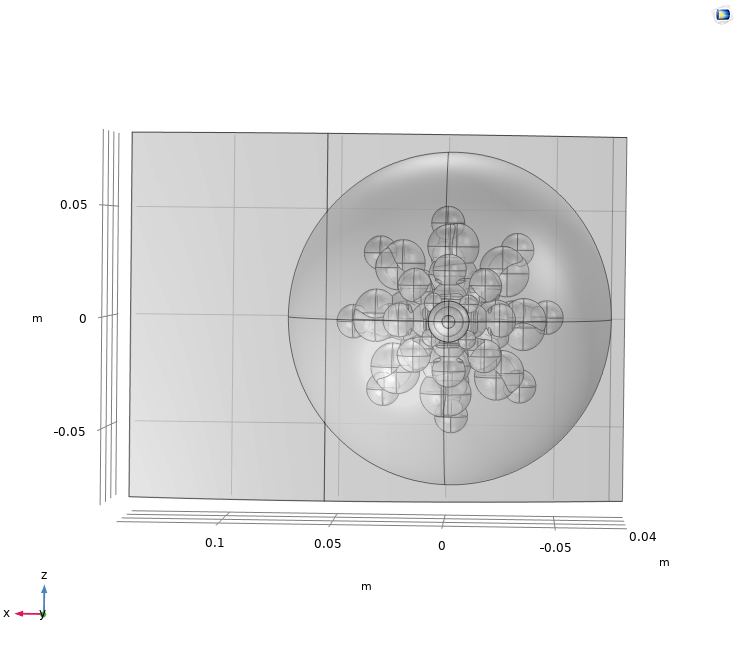
\includegraphics[width=\linewidth]{Figures/model_pictures/stage3_glandular/stage3_glandular_ref_anterior_offset055.png}}{\fbox{\parbox[c][0.24\textheight][c]{0.9\linewidth}{\centering Placeholder: Stage 3 reference anterior view}}}
\caption{Anterior overview}
\end{subfigure}
\hfill
\begin{subfigure}{0.48\linewidth}
\centering
\IfFileExists{Figures/model_pictures/stage3_glandular/stage3_glandular_ref_lateral_slice.png}{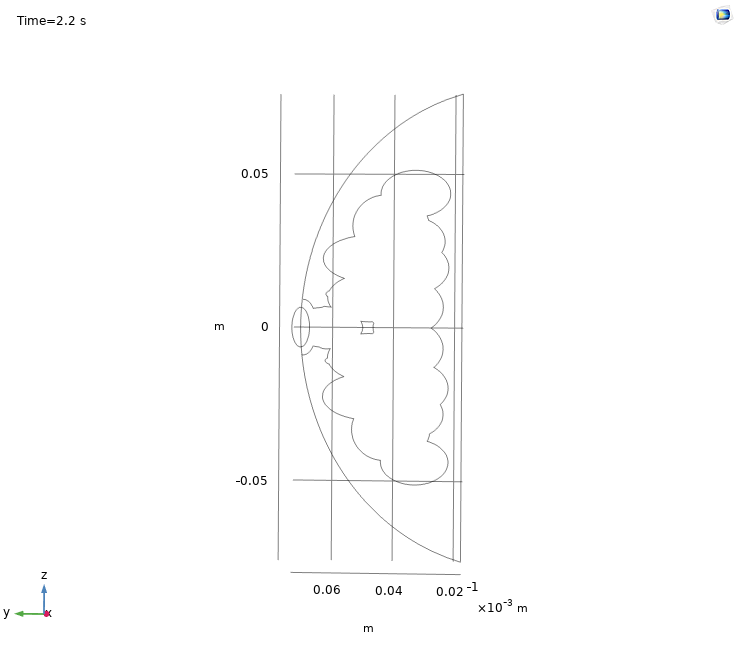
\includegraphics[width=\linewidth]{Figures/model_pictures/stage3_glandular/stage3_glandular_ref_lateral_slice.png}}{\fbox{\parbox[c][0.24\textheight][c]{0.9\linewidth}{\centering Placeholder: Stage 3 reference sagittal slice}}}
\caption{Sagittal slice}
\end{subfigure}
\caption{Current reference model used as the anatomical baseline for later sensitivity studies. The figure shows the selected xoffset055 chestwall route combined with the realistic glandular lobule distribution.}
\label{fig:mm_reference_geometry}
\end{figure}

Stage 4 and Stage 5 were structured as matched controls. The Stage 4 reference intentionally keeps asymmetry disabled so that later asymmetry cases can be compared against it. The Stage 5 no-Cooper case intentionally keeps the same geometry and disables Cooper support so that later stable Cooper variants can be compared against a matched control.

\subsection{Dynamic input}

The standard transient input is a fixed-support acceleration pulse with amplitude 0.25g, duration 0.60 s, and mass damping alpha = 60 s$^{-1}$. This input is meant to be a mild platform- or torso-like acceleration for controlled model comparison. It should not be described as a direct physical reproduction of a jump or as an exact Early Warning Scan protocol. Its role is to produce a gentle, reproducible dynamic displacement and stress response.

\subsection{Material modelling}

The source-case material settings contain adipose, glandular, skin, support, and optional tumor/lesion parameters. The tissue parameters are based on Mooney--Rivlin-style coefficients and density values, while the COMSOL implementation maps these into the current material scaffold used by the Java builder. Literature values for breast soft tissue vary strongly with test protocol, tissue type, loading state, and subject characteristics \cite{Samani2007,Ramiao2016,Teixeira2023,Chen2025}. The material set is therefore used as a controlled reference for sensitivity studies, not as a patient-specific calibration.

The current Stage 6 tumor implementation is an analytic material overlay. A spherical \texttt{tumor\_mask} is defined from radius and position parameters. Inside that mask, density and Mooney--Rivlin coefficients are modified locally in adipose and glandular material expressions. This does not create a separate COMSOL tumor domain and does not create a separate \texttt{mat\_tumor} material. Tumor-region metrics are computed by mask-weighted volume integrations over the breast union. This route is deliberately used as a first stiffness and location sensitivity because it avoids fragile Boolean operations while still allowing local displacement and stress metrics to be exported.

The initial lesion sizes are 6 mm, 12 mm, and 20 mm diameter. These span small early lesions, a mid-range screening-style lesion, and an upper T1-size diagnostic sensitivity; they also align with earlier DIET phantom work that tested 5, 10, and 20 mm stiff inclusions \cite{NCI_TNM,Kashif2013}. The first location set includes central, subareolar, posterior/chestwall-proximal, and upper-outer candidates. The upper-outer candidate is emphasized because breast-cancer quadrant studies report this as the most frequent tumor site, while anatomical-distribution work also describes the upper-outer predominance as non-random \cite{Rummel2015,Yu2017}. Additional surface-proximal candidates were added because tumor-to-skin or tumor-to-dermis distance is clinically evaluated in superficial breast tumors \cite{Brandao2023,Yur2023}. The current model keeps these as internal spherical inclusions; a visible surface bulge would require a separate geometry-deformation case and is therefore not part of the first report-ready Stage 6 route.

Tumor shape is kept spherical in the current implementation. Imaging descriptors such as round, oval, irregular, and spiculated masses are clinically relevant in BI-RADS terminology \cite{ACRBIRADS,UCLABIRADS}, but ellipsoidal or irregular lesion shapes would require extending the analytic mask or adding separate visual geometry. Those shapes are therefore treated as future Stage 6B sensitivity cases rather than as current results.

\begin{figure}[H]
\centering
\begin{subfigure}{0.48\linewidth}
\centering
\IfFileExists{Figures/model_pictures/stage6_tumor/stage6_tumor_small_upper_outer_leftlateral.png}{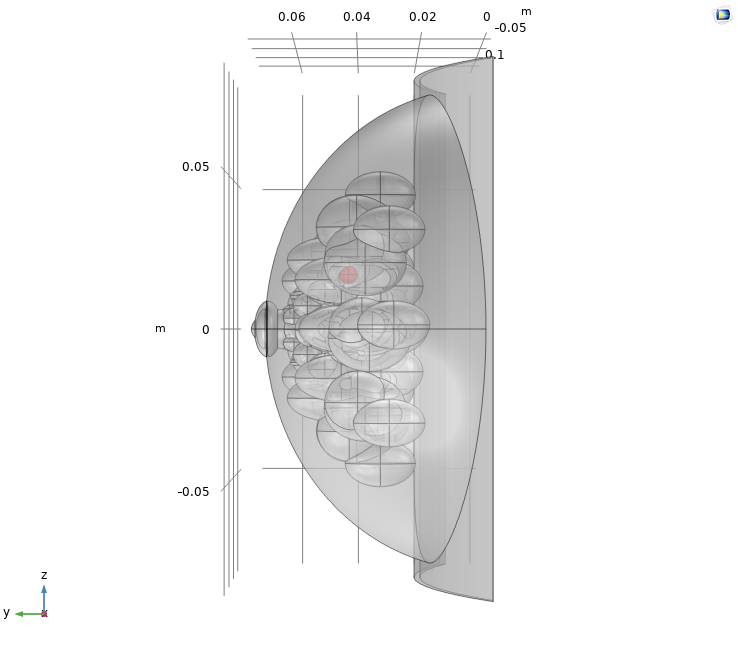
\includegraphics[width=\linewidth]{Figures/model_pictures/stage6_tumor/stage6_tumor_small_upper_outer_leftlateral.png}}{\fbox{\parbox[c][0.24\textheight][c]{0.9\linewidth}{\centering Placeholder: small upper-outer tumor view}}}
\caption{Small upper-outer candidate}
\end{subfigure}
\hfill
\begin{subfigure}{0.48\linewidth}
\centering
\IfFileExists{Figures/model_pictures/stage6_tumor/stage6_tumor_large_central_sideview.png}{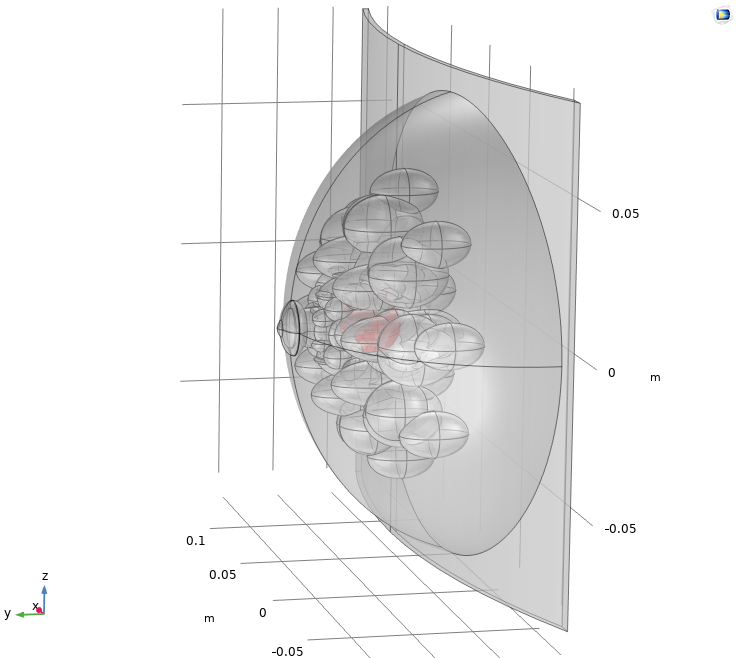
\includegraphics[width=\linewidth]{Figures/model_pictures/stage6_tumor/stage6_tumor_large_central_sideview.png}}{\fbox{\parbox[c][0.24\textheight][c]{0.9\linewidth}{\centering Placeholder: large central tumor view}}}
\caption{Large central candidate}
\end{subfigure}
\caption{Visual examples of the Stage 6 spherical tumor-mask screening route. These images are used to document placement and scale; quantitative interpretation still depends on completed tumor-mask post-processing metrics.}
\label{fig:mm_stage6_tumor_visual}
\end{figure}

\subsection{Cooper ligament surrogate}

Cooper ligament support is currently treated as a mechanical support sensitivity rather than an exact anatomical reconstruction. The matched no-Cooper control is useful, but the default Cooper run failed almost immediately because of nonlinear solver/out-of-core problems. For that reason, the current Tier 1 comparison does not show a reliable Cooper effect. Future Cooper tests should start with milder support variants and should be evaluated first as build-only or short diagnostic runs before overnight solves.

\subsection{Mesh, build, and solver checks}

The pipeline supports generate-only, build-only, full run, and postprocess-only workflows. For new geometry or lesion cases, build-only is used first to verify geometry construction, selections, source-case expansion, and generated Java builder output without starting a heavy solve. This is especially important for Stage 6, where the tumor location must be checked visually and numerically before interpreting displacement or stress results.

The generated output includes resolved TOMLs, single-file cases, source-case expansion files, COMSOL build plans, selection hints, Java builder scripts, solver logs, metrics JSON files, time-series CSV files, and screenshot folders. Large generated MPH files, recovery files, COMSOL configuration caches, and full run folders are treated as local artefacts rather than GitHub-ready repository content.

\subsection{Post-processing and evaluation metrics}

The post-processing route exports breast, glandular, adipose, and tumor-mask metrics when available. The main quantities are total breast volume, glandular volume fraction, average and maximum displacement, signed surface displacement, nipple/landmark displacement, average and maximum von Mises stress, tissue stress, and time-series evolution. For tumor cases, additional mask-based metrics include tumor volume, tumor-region displacement, and tumor-region stress.

The Tier 1 comparison uses existing COMSOL outputs only. Stage 1 is interpreted as the motion sanity baseline, Stage 2 as the first fair anatomical baseline, Stage 3 as the realistic glandular reference, Stage 4 as the no-asymmetry control, and Stage 5 as the no-Cooper control. Stage 6 should only be added to formal comparison plots after complete and meaningful tumor metrics are available.
